% LATER: adicionar subseção de modelagem do problema
% LATER: adicionar gráfico (fluxo por tempo) em tratamento de dados.

Como visto anteriormente, congestionamentos nas cidades tendem a piorar com o aumento de carros. Sendo assim, é importante pensar em métodos para evitar ou aliviar o alto fluxo de carros. Neste contexto, este trabalho propõe uma arquitetura de predição de tráfego baseado em \acrshort{GAN} com \acrshort{LSTM} para prever, utilizando dados de fiscalização eletrônica, o fluxo futuro das vias monitoradas. No caso, a previsão seria para curto e médio período (5, 10, 15, 30, 60, 120, 150 minutos). No intuito de fornecer essa informação para os cidadãos, para que estes possam se organizar melhor e se distribuir na malha rodoviária. No restante deste capítulo serão detalhados as etapas da metodologia.

\section{Coleta de dados}
Para predizer o tráfego será necessário a série temporal que corresponde ao fluxo de uma via. Os dados utilizados nesse trabalho foram coletados pelo \acrfull{DETRAN}\footnote{http://www.detran.df.gov.br/} do \acrfull{DF} de maio de 2018 a junho de 2018 de 4 vias diferentes. Para cada carro é registrado uma entrada contendo o identificador do equipamento, a data e hora, a faixa em que atravessou, a velocidade, a velocidade limite e o tamanho, como apresentado na Tabela \ref{table:data}.

\begin{table}[h]
    \begin{tabular}{ccccccc}
    \toprule
    \multicolumn{1}{l}{\textbf{Id Equipamento}} & \multicolumn{1}{l}{\textbf{Data}} & \multicolumn{1}{l}{\textbf{Hora}} & \multicolumn{1}{l}{\textbf{Faixa}} & \multicolumn{1}{l}{\textbf{km/h}} & \multicolumn{1}{l}{\textbf{km/h Max}} & \multicolumn{1}{l}{\textbf{Tamanho}} \\ 
    \midrule
    RSI128 & 2016/05/01 & 00:00:09 & 1 & 20 & 60 & 0 \\
    RSI131 & 2016/05/01 & 00:00:09 & 2 & 45 & 60 & 1.1 \\
    RSI132 & 2016/05/01 & 00:00:09 & 1 & 40 & 60 & 0 \\
    RSI131 & 2016/05/01 & 00:00:10 & 1 & 35 & 60 & 0.5 \\ 
    \bottomrule
    \end{tabular}
    \label{table:data}
    \caption{Exemplo dos dados recebidos coletados pelo \acrshort{DETRAN}}
\end{table}

Os dados foram obtidos do equipamento de fiscalização eletrônica, os quais estão instalados em vias semafóricas. Por este motivo, é possível identificar momentos curtos onde não há fluxo de carros. Além disso, alguns dos equipamentos sofreram manutenção, resultando em alguns momentos mais longos sem registro de tráfego.

\begin{figure}[t]
    \centering
    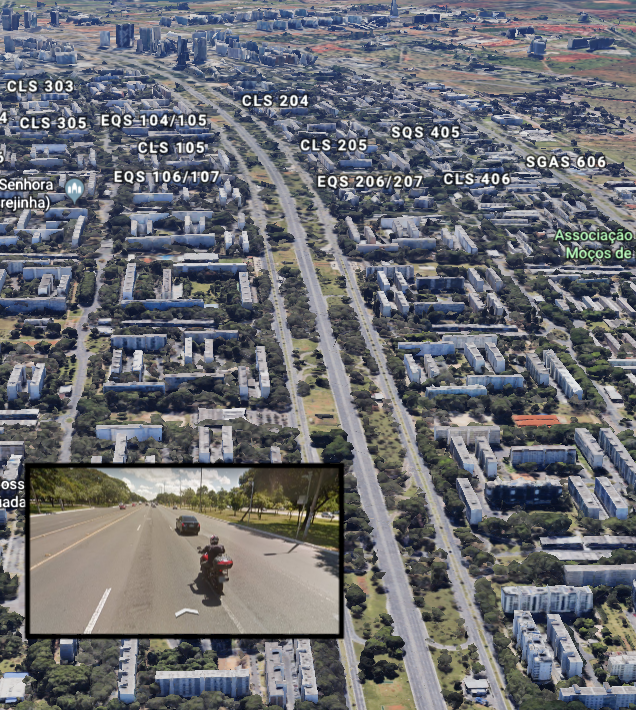
\includegraphics[scale=0.5]{street.png}
    \label{figure:eixo}
    \caption{Visão espacial do eixo monumental em Brasília}
\end{figure}

\section{Pré-Processamento dos Dados}

O tráfego é afetado por variáveis temporais (horários de pico), espaciais (centros metropolitanos) e aleatórias (acidentes, chuvas). Porém, devido a dificuldade de prever os dados aleatórios, é mais comum na literatura encontrar pesquisas que trabalham apenas com os dados temporais e espaciais. Sendo assim, assume-se que (i): existe uma tendência do fluxo se repetir e (ii): eventos aleatórios não afetam a tendência do fluxo.

Nesta etapa será feita uma avaliação dos dados, pois alguns deles não são muito relevantes para a pesquisa, ou não foram medidos de forma precisa, como por exemplo o tamanho do veículo e, portanto, serão removidos. Além disso, podemos extrair mais informações dos dados que recebemos, tal como calcular o dia da semana em que o dado foi registrado e verificar se é um feriado ou dia comemorativo. Isso permitirá uma análise melhor da relação entre dia da semana e intensidade do fluxo nas vias.

Também será preciso lidar com as manutenções que as infraestruturas podem ter no tempo da série temporal que coletamos, e para isso podemos preencher com aproximações ou simplesmente diminuir a quantidade de dados coletados para que não exista mais a falha.

\section{Implementação}

Nesta etapa serão implementados as duas arquiteturas, isto é, a arquitetura proposta (\acrshort{GAN} com \acrshort{LSTM}) e o estado da arte (\acrshort{SLSTM}). Para tal, usaremos do \textit{framework} \textit{TensorFlow}, visto que este é o framework com suporte para aprendizado de máquina mais utilizado dentre os desenvolvedores, segundo um \textit{survey} feito em 2018 pelo \textit{StackOverflow} \cite{stack_2018}.

Nesta fase serão utilizados apenas dois terços dos dados obtidos, o restante dos dados serão utilizados posteriormente como teste. Esses dados de treino serão divididos em diversos blocos contendo um intervalo de tempo contínuo. Esses blocos serão usados como entrada tanto para o gerador da arquitetura proposta quanto para o estado da arte. Além disso, o gerador e o estado da arte terão a mesma saída, uma série temporal que seja a continuação da série de entrada, predizendo os próximos t minutos. Já o discriminador terá como entrada tanto a saída do gerador ,quanto a série temporal real, retornando como saída a probabilidade de que o resultado do gerador seja real.

Para cada tentativa de predição diferente, isto é, tentar predizer 5, 10, 15, 30, 60, 120 ou 150 minutos, será feito um novo treinamento na arquitetura. Assim, treinaremos as redes neurais especificamente para o intervalo de tempo que ela deve prever naquele momento.

\section{Avaliação Final}

Nessa fase serão utilizados os 1/3 dos dados restantes. Para cada treino da fase de implementação, serão utilizados esses dados de teste para verificar qual dos dois modelos (o modelo proposto pelo trabalho, ou o estado da arte) foi capaz de prever melhor o fluxo de carros futuro. Ou seja, os dados de teste serão comparados com as previsões dos dois modelos e a acurácia de ambos será verificada utilizando \acrshort{MAE}, \acrshort{MRE} e \acrshort{RMSE}. Além disso, também será utilizado o método de \textit{K-Fold Cross Validation} para a estimação dos parâmetros e validação da metodologia como um todo.
